%!TEX root = MemoireZelliges_simple.tex

\chapter{Étude physique d'un zellige blanc (\bdx{6532})}
%======================================================================

\section{Description -- État de surface}
%----------------------------------------------------------------------

Cet échantillon (\fref{dessin:6532}), de forme parallélépipédique, 
est une pièce de céramique glaçurée de couleur blanche. Il provient 
du \PaM (\siecle{xvii}) de Meknès. Il est chamfreiné. Les traces 
d'encre violacée résultent de l'indexation de l'échantillon au Maroc.

\begin{itemize}
  \item \DimText : \SI{55x50x20}{\mm}
  \item \emph{Masse} : \SI{76.0}{\g}
\end{itemize}


\begin{figure}[htb]
  \begin{minipage}[t]{0.5\textwidth}
    \centerfloat
    \vspace*{0pt}
    % \fakeimg{Dessin de l'échantillon : Vue de dessus}
    \includegraphics[scale=1]{BDX6532_dessus}
    \subcaption{Vue de dessus \label{dessin:6532_dessus}}
  \end{minipage}%
  \quad%
  \begin{minipage}[t]{0.5\textwidth}
    \centerfloat
    \vspace*{0pt}
    % \fakeimg{Dessin de l'échantillon : Lame}
    \includegraphics[scale=1]{BDX6532_lame}
    \subcaption{Lame étudiée \label{dessin:6532_lame}}
  \end{minipage}

  \bigskip

  \begin{minipage}[t]{0.5\textwidth}
    \centerfloat
    \vspace*{0pt}
    % \fakeimg{Dessin de l'échantillon : Coupe}
    \includegraphics[scale=1]{BDX6532_coupe}
    \subcaption{Vue en coupe \label{dessin:6532_coupe}}
  \end{minipage}%
  \quad%
  \begin{minipage}[t]{0.5\textwidth}
    \vspace*{0pt}
    Légende :

    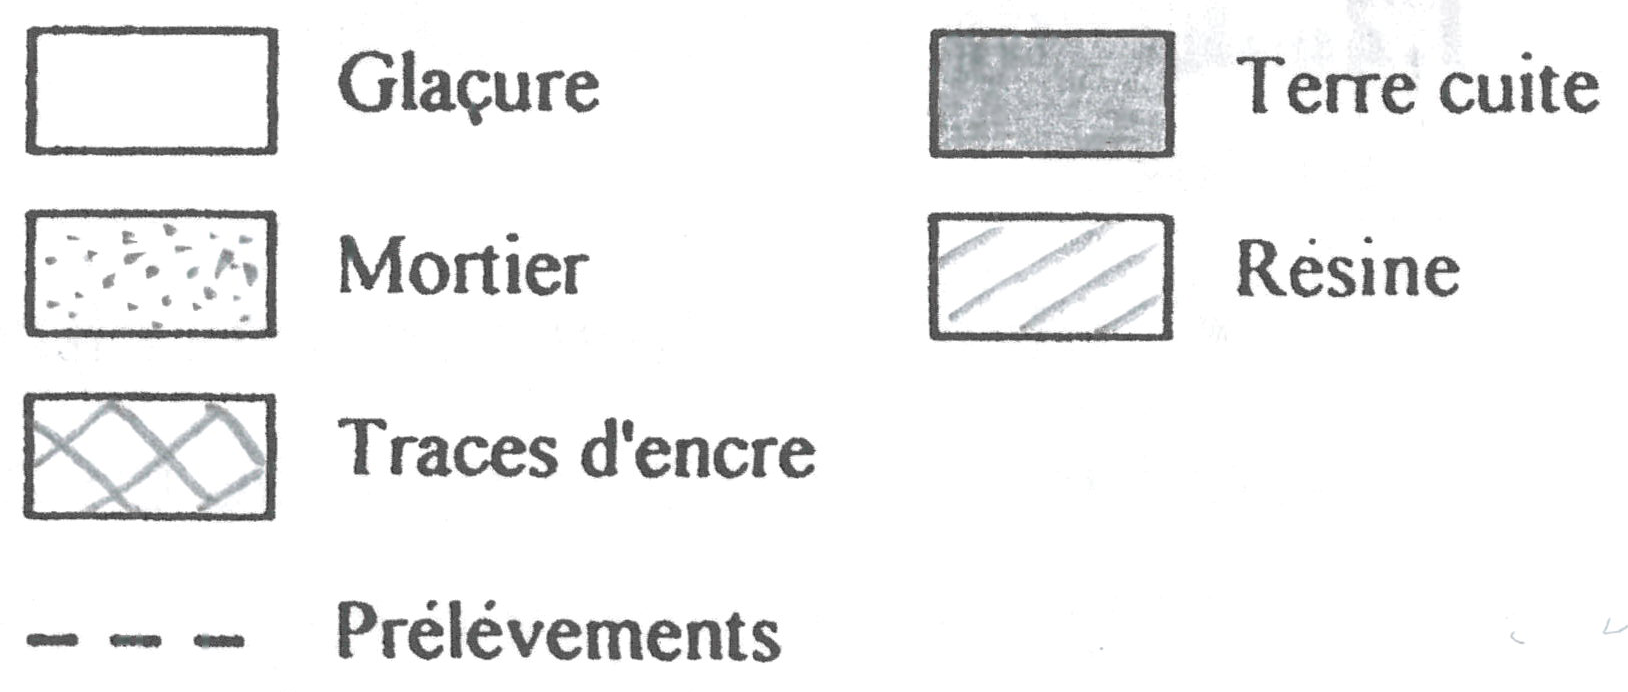
\includegraphics[scale=1]{dessin_legende}
    % \begin{itemize}
    %   \item Terre cuite
    %   \item Glaçure
    %   \item Résine
    %   \item Mortier
    %   \item Traces d'encre
    %   \item Prélévements
    % \end{itemize}
  \end{minipage}
  \caption{\legendeE}
  \label{dessin:6532}
\end{figure}

L'observation de la surface de la glaçure (\fref{surf:6532}) montre 
qu'elle contient des bulles, des picots, présente des rayures et 
contient des cristaux non fondus.

Le support de terre cuite est de couleur rosé, de granulométrie 
fine, peu poreux et contient de nombreuses inclusions de tailles 
et de couleurs variées.

\begin{figure}[htb]
  Etat de surface
  \caption{\legendeE 
           État de surface de la glaçure (Gr=30, \zone{\sim4.3x3.2}{\mm}). Elle contient des bulles, des 
           picots, des cristaux non fondus et présente des rayures.}
  \label{surf:6532}
\end{figure}


\section{Étude de la couleur}
%----------------------------------------------------------------------

\subsection{Identification des ions chromogènes}
%~~~~~~~~~~~~~~~~~~~~~~~~~~~~~~~~~~~~~~~~~~~~~~~~~~~~~~~~~~~~~~~~~~~~~~
\begin{figure}[htb]
  \begin{plotspectre}
    \addplot [thick, LightGoldenrod] 
       table [x=lambda, y=6532gla] {\gladata} ;
    \addplot [thick, FireBrick] 
       table [x=lambda, y=6532tc] {\tcdata} ;
  \end{plotspectre}
  \caption{\legendeE 
           Spectre d'\AO en mode réflexion diffuse de la glaçure. Le spectre ne présente pas de bande d'absorption particulière dans le visible et ne permet donc pas l'identification d'éléments chromogènes particuliers.}
  \label{spectre:6532}
\end{figure}

Le spectre d'\AO en mode réflexion diffuse de la glaçure (\fref{spectre:6532}) montre une absorption faible dans l'ensemble du domaine du visible et ne permet pas l'identification d'éventuels éléments chromogènes.

\subsection{Mesure physique de la couleur}
%~~~~~~~~~~~~~~~~~~~~~~~~~~~~~~~~~~~~~~~~~~~~~~~~~~~~~~~~~~~~~~~~~~~~~~
Les coordonnées \trichro s correspondant aux espaces \Yxy et \Lab ont été calculées pour la glaçure et de la terre cuite, à partir de leurs spectres d'\AO (\tref{saotab:6532}). La longueur d'onde dominante de la glaçure ($\lambda_D=\SI{575.30}{\nm}$) correspond au domaine du jaune \autocite{Kelly_1976} et la pureté d'excitation indique une couleur peu saturée ($P_e=\SI{13.84}{\percent}$). L'apparence blanche de la glaçure est due à sa forte réflectance ($Y=\num{50.011}$).

La \fref{colorfig:6532} montre la localisation des coordonnées 
chromatiques de la glaçure dans les espaces \Yxy et \Lab.

La longueur d'onde dominante ($\lambda_D=\SI{581.15}{\nm}$) de la 
terre cuite correspond au jaune orange \autocite{Kelly_1976}. La 
pureté d'excitation est assez faible ($P_e=\SI{24.58}{\percent}$) 
et la réflectance assez élevée ($Y=\num{35.676}$), on peut donc 
parler d'une couleur claire.

\begin{table}
  \begin{saotab}
      \saolgna{Glaçure}{575.30}{13.84}
              {50.011}{0.336}{0.355}
              {76.076}{-0.635}{11.486} &
      \saolgnb{Jaune clair}{Jaune}{575}{580}{\footnotemark{}}
    \tabularnewline
      \saolgna{Terre cuite}{581.15}{24.58}
              {35.676}{0.370}{0.370}
              {66.272}{5.871}{19.355} &
      \saolgnb{jaune orange clair}{jaune orange}{580}{585}
              {\footnotemark{}}
    \tabularnewline
  \end{saotab}
  \caption{\legendeE 
           Coordonnées chromatiques dans les systèmes \Yxy et \Lab 
           et longueur d'onde dominante (illuminant D65, \ang{2},
           \SIrange{400}{700}{\nm}).}
  \label{saotab:6532}
\end{table}
\footnotetext{\autocite{Kelly_1976}}
\footnotetext{\autocite{Kelly_1976}}

\begin{figure}[htb]
  \newcommand{\samplename}{6532gla}
  \newcommand{\samplecolor}{LightGoldenrod}
  \begin{minipage}[t]{0.37\paperwidth}
    \begin{plotYxy}
      \plotYxyPaV ;
      \plotYxyIlluminant ;
      \plotYxySample{\samplename}{\samplecolor} ;
      \plotYxyLigne{\samplename} ;
      \plotYxyAnnot{\samplename}{south west} ;
    \end{plotYxy}
    \subcaption{espace \trichro \Yxy. La longueur d'onde 
                dominante de la glaçure est de \SI{575.300}{\nm}. 
                Elle est dans le domaine du jaune, la couleur est 
                assez peu saturée.}
  \end{minipage}%
  \qquad%
  \begin{minipage}[t]{0.37\paperwidth}
    \begin{plotLab}
      \plotLabSample{\samplename}{\samplecolor} ;
    \end{plotLab}
    \subcaption{espace \trichro \Lab. Le point représentatif de 
                la couleur de la glaçure est sur la ligne du jaune.}
  \end{minipage}%
  \caption[\bdx{6532}\ -- Espaces \trichro s]
          {\legendeE Analyse chromamétrique de la glaçure.}
  \label{colorfig:6532}
\end{figure}


\section{Étude de la texture de la glaçure et de la terre cuite sur 
         une section polie}
%----------------------------------------------------------------------

\subsection{Observation en lumière naturelle}
%~~~~~~~~~~~~~~~~~~~~~~~~~~~~~~~~~~~~~~~~~~~~~~~~~~~~~~~~~~~~~~~~~~~~~~
\begin{figure}[htb]
  \begin{minipage}[t]{0.4\textwidth}
    \fakeimg{lum. nat.}
    \subcaption{Lumière naturelle \label{texture:6532_LN}}
  \end{minipage}
  \begin{minipage}[t]{0.4\textwidth}
    \fakeimg{Cathodo}
    \subcaption{\CL \label{texture:6532_CL}}
  \end{minipage}
  \caption{\legendeE 
           Observation de la texture en section sur une surface de 
           \SI{2.6x1.9}{\mm}.}
  \label{texture:6532}
\end{figure}

L'examen en section (\fref{texture:6532_LN}) montre que la 
glaçure est opaque, colorée dans la masse et qu'elle adhère bien au 
support céramique. La terre cuite contient de nombreuses inclusions 
de tailles et de couleurs diverses, réparties de manière homogène.

La limite entre la glaçure et la terre cuite semble très nette.

\subsection{Observation en \CL}

La glaçure n'est pas luminescente (\fref{texture:6532_CL}). 
Cependant, on observe à sa surface des luminescences mauve.

La terre cuite présente une luminescence à dominante mauve ainsi que 
des luminescences ponctuelles rouges et bleues se répartissant de 
manière homogène dans tout le matériau.

On ne distingue aucune luminescence à l'interface terre cuite-glaçure.

\subsection{Observation en \MEB[ie]}
%~~~~~~~~~~~~~~~~~~~~~~~~~~~~~~~~~~~~~~~~~~~~~~~~~~~~~~~~~~~~~~~~~~~~~~
La glaçure (\fref{MEB:6532_img}) a une épaisseur moyenne de \SI{260}{\um}. Elle contient des bulles et des cristaux non fondus, identifiés comme des quartz par \carto de \RX (\fref{MEB:6532_carto_tcgla}) et analyses ponctuelles par \spectro de \RX.

\begin{figure}[htb]
  \fakeimg{Texture au MEB, retrodiff}
  \caption{\legendeE 
           Observation de la texture au \MEB, en mode \ERD. 
           Ensemble glaçure/terre cuite. La barre d'échelle mesure 
           \SI{200}{\um} (\zone{500x400}{\um}).}
  \label{MEB:6532_img}
\end{figure}

On remarque également des cristaux de quartz non fondus formant un liseré continu à la surface de la glaçure. Ils sont responsables de la luminescence mauve détectée dans cette zone en \CL.

En \carto de \RX (\fref{MEB:6532_carto_tcgla}), on distingue la répartition homogène de l'étain, sous forme de grains de cassitérite (\ce{SnO2}), dans toute la glaçure.

Des grains de quartz de faible granulométrie (\SI{\sim10}{\um}) ont pu être ajoutés au mélange glaçurant en même temps que la cassitérite. On peut penser qu'ils participent à l'opacification de la glaçure par un effet de diffusion de la lumière.

\begin{figure}[htb]
  \fakeimg{Texture au MEB, carto tc/gla}
  \caption{\legendeE 
           Observation de la texture au \MEB, \carto de \RX de l'ensemble glaçure/terre cuite (Gr=190, \zone{580x475}{\um}).}
  \label{MEB:6532_carto_tcgla}
\end{figure}

\begin{figure}[htb]
  \fakeimg{Texture au MEB, carto tc}
  \caption{\legendeE 
           Observation de la texture au \MEB, en mode \ERD. 
           Zone d'interface. La barre d'échelle mesure \SI{50}{\um} 
           (\zone{185x175}{\um}).}
  \label{MEB:6532_img_int}
\end{figure}

À l'interface glaçure-terre cuite (\fref{MEB:6532_img_int}), on 
distingue des cristaux de néoformation de forme aciculaire.

La terre cuite (\fref{MEB:6532_carto_tc}) contient des inclusions de 
quartz (\ce{SiO2}) et d'alumino-silicates calco-potassiques.

\begin{figure}[htb]
  Texture au MEB, carto tc (fig 25)
  \caption{\legendeE 
           Observation de la texture au \MEB, \carto de \RX de la terre cuite (Gr=140, \zone{785x640}{\um}).}
  \label{MEB:6532_carto_tc}
\end{figure}


\section{Composition élémentaire de la glaçure}
%----------------------------------------------------------------------

Le \tref{compelem:6532_gla} présente la composition élémentaire de 
la glaçure blanche obtenue par \EDS.

Il s'agit d'une glaçure plombifère (\SI{47.88}{\percent} de \ce{PbO}) 
opacifiée à l'étain (\SI{5.19}{\percent} de \ce{SnO2}). La très faible 
teneur en fer (\SI{0.90}{\percent} de \ce{Fe2O3}) ne suffit pas à 
colorer la glaçure.

\begin{table}
  \begin{cartotab}
      \cartolgn{SiO2}{38.59}{1.43} &
      \cartolgn{CaO}{3.77}{0.06}   &
      \cartolgn{Al2O3}{1.65}{0.15} &
      \cartolgn{MgO}{0.60}{0.04}
    \tabularnewline
      \cartolgn{Na2O}{0.28}{0.04}  &
      \cartolgn{K2O}{0.94}{0.06}   &
      \cartolgn{Fe2O3}{0.90}{0.13} &
      \cartolgn{PbO}{47.88}{1.43}
    \tabularnewline
      \cartolgn{SnO2}{5.19}{0.43} &
      \cartolgnnd{CuO}            &
      \cartolgnnd{CoO}            &
      \cartolgnnd{MnO}
    \tabularnewline
      \cartolgnnd{Cr2O3}          &
      \cartolgnnd{ZnO}            &
      \cartolgnnd{Sb2O3}          &
      \cartolgnnd{TiO2}
    \tabularnewline
      \cartolgnnd{S}              &
      \cartolgnnd{P2O5}           &
      \cartolgn{Cl}{0.22}{0.08}   &
      \cartolgnnd{As2O5}
    \tabularnewline
  \end{cartotab}
  \caption{\legendeE 
           Analyse quantitative par \EDS. Composition élémentaire de la glaçure blanche sur une surface de \SI{108x88}{\um} (\PMO).}
  \label{compelem:6532_gla}
\end{table}


\section{Étude de la terre cuite support}
%----------------------------------------------------------------------

\subsection{Composition élémentaire}
%~~~~~~~~~~~~~~~~~~~~~~~~~~~~~~~~~~~~~~~~~~~~~~~~~~~~~~~~~~~~~~~~~~~~~~
\begin{table}
  \begin{cartotab}
      \cartolgn{SiO2}{51.96}{1.62} &
      \cartolgn{CaO}{19.46}{0.96} &
      \cartolgn{Al2O3}{14.03}{0.61} &
      \cartolgn{MgO}{3.47}{0.27}
    \tabularnewline
      \cartolgn{Na2O}{0.53}{0.05} &
      \cartolgn{K2O}{1.43}{0.16} &
      \cartolgn{Fe2O3}{7.52}{0.36} &
      \cartolgnnd{PbO}
    \tabularnewline
      \cartolgnnd{SnO2} &
      \cartolgnnd{CuO} &
      \cartolgnnd{CoO} &
      \cartolgnnd{MnO}
    \tabularnewline
      \cartolgnnd{Cr2O3} &
      \cartolgnnd{ZnO} &
      \cartolgnnd{Sb2O3} &
      \cartolgn{TiO2}{0.81}{0.10}
    \tabularnewline
      \cartolgn{S}{0.15}{0.03} &
      \cartolgn{P2O5}{0.57}{0.23} &
      \cartolgn{Cl}{0.06}{0.02} &
      \cartolgnnd{As2O5}
    \tabularnewline
  \end{cartotab}
  \caption{\legendeE Analyse quantitative par \EDS. Composition élémentaire de la terre 
           cuite sur une surface de \SI{2160x1752}{\um} (\PMO).}
  \label{compelem:6532_tc}
\end{table}

La terre cuite (\tref{compelem:6532_tc}) est riche en calcium. 
Sa coloration ocre rosé est due au \ce{Fe^3+} (\SI{7.52}{\percent} 
de \ce{Fe2O3}) en atmosphère de cuisson oxydante 
\autocite{Echallier_1984}. Ici encore, c'est l'excès de fer, non 
piégé dans les phases haute température, qui colore la terre cuite.

\subsection{Composition \cristallo}
%~~~~~~~~~~~~~~~~~~~~~~~~~~~~~~~~~~~~~~~~~~~~~~~~~~~~~~~~~~~~~~~~~~~~~~
Le principal composé cristallisé mis en évidence par \DX sur poudre (\fref{DRX:6528}) est le quartz (\ce{SiO2}), responsable 
de la luminescence mauve de la terre cuite. On relève également la
présence, à des teneurs plus faibles, de calcite (\ce{CaCO3}) pouvant 
correspondre aux émissions rouges détectées en \CL, d'anorthite 
(\ce{CaAl2Si2O8}), de diopside alumineux 
(\ce{Ca(Mg{,}Al)(Si{,}Al)2O6}) et de gehlénite (\ce{Ca2Al2SiO7}). 
Ces trois derniers cristaux peuvent être responsables des émissions 
bleues détectées en \CL.

La présence d'anorthite, de diopside alumineux et de gehlénite, 
trois phases se développant à haute température, laisse penser que 
la température de cuisson maximale de la céramique se situe autour 
de \SIrange[range-phrase=\ à\ ]{900}{950}{\degC}.

\begin{figure}[htb]
  \includegraphics[width=\textwidth]{BDX6532_DX}
  \caption{\legendeE 
           \DX sur poudre de la terre cuite. 
           Mise en évidence de la présence de quartz (Q), calcite (C), 
           gehlénite (G), anorthite (A), diopside (D).}
  \label{DRX:6532}
\end{figure}


\section{Sur la présence et l'identification de cristaux de 
         dévitrification}
%----------------------------------------------------------------------

On distingue, dans la zone d'interface terre cuite/glaçure, des cristaux de forme aciculaire. Ce sont des cristaux de dévitrification croissant pendant le refroidissement lent de la glaçure à partir de germes formés à haute température. Des analyses ponctuelles par \EDS ont montré (\tref{compelem:6532_cx}) que ces cristaux sont des alumino-silicates de calcium et de plomb.

\begin{table}
  \begin{cartotab}
      \cartolgn{SiO2}{39.64}{3.68} &
      \cartolgn{CaO}{5.85}{0.63}   &
      \cartolgn{Al2O3}{4.02}{0.61} &
      \cartolgn{MgO}{0.80}{0.28}
    \tabularnewline
      \cartolgn{Na2O}{0.25}{0.10}  &
      \cartolgn{K2O}{1.07}{0.09}   &
      \cartolgn{Fe2O3}{1.83}{0.16} &
      \cartolgn{PbO}{43.92}{4.89}
    \tabularnewline
      \cartolgn{SnO2}{2.14}{1.39} &
      \cartolgnnd{CuO}            &
      \cartolgnnd{CoO}            &
      \cartolgnnd{MnO}
    \tabularnewline
      \cartolgnnd{Cr2O3} &
      \cartolgnnd{ZnO}   &
      \cartolgnnd{Sb2O3} &
      \cartolgn{TiO2}{0.24}{0.07}
    \tabularnewline
      \cartolgnnd{S}            &
      \cartolgnnd{P2O5}         &
      \cartolgn{Cl}{0.24}{0.11} &
      \cartolgnnd{As2O3}
    \tabularnewline
  \end{cartotab}
  \caption{\legendeE Analyse quantitative par \EDS. Composition élémentaire des cristaux 
           de dévitrification par analyses ponctuelles 
           (\SI{1}{\um\squared}) (\PMO).}
  \label{compelem:6532_cx}
\end{table}


\section{Étude des altérations de la glaçure}
%----------------------------------------------------------------------

Aucune figure d'altération n'a été mise en évidence dans la glaçure, 
ni visuellement, ni en \MEB[ie] (MEB).


\section{Bilan}
%----------------------------------------------------------------------

Cet échantillon est donc une pièce de céramique portant une glaçure 
plombifère dont la coloration blanche est due à une opacification à 
l'étain. La présence de fins cristaux non fondus de quartz à sa 
surface participe aussi à cette opacification.

Son support de terre cuite est de type calcique. Sa coloration 
ocre-rose est due à la présence de \ce{Fe^3+} en atmosphère de 
cuisson oxydante.

Sa composition \cristallo (quartz, calcite, diopside, gehlénite, anorthite) laisse penser qu'elle a été cuite à une température de l'ordre de \SIrange[range-phrase=\ à\ ]{900}{950}{\degC}.

À l'interface glaçure-terre cuite, on n'observe pas de luminescence. 
Cependant, cette zone renferme des cristaux de dévitrification 
identifiés comme des des alumino-silicates de calcium et de plomb. 
Le faible développement de cette zone laisse envisager l'application 
du mélange glaçurant sur une terre cuite.

La glaçure ne présente pas de figure d'altération d'origine chimique 
mais une usure mécanique de surface.